\begin{abstract}
hello
\end{abstract}

\section{Introduction}
For many years, many standalone Internet of Things (IoT) platforms have been developed and deployed in different domains. The recent trend, however, is to evolve towards a globally unified IoT platform, in which billions of objects connect to the Internet, available for interactions among themselves, as well as interactions with many different applications across boundaries of administration and domains. 


Building a unified IoT platform, however, poses a set of unique challenge and requirement on the underlying network and systems.
\begin{itemize}
\vspace{1mm}\item{\bf Identity}:
To realize a unified IoT platform, the first step is the capability to assign names that are unique within the scope and lifetime of each device, data items generated by these devices, or a group of devices towards a common objective.
\vspace{1mm}\item{\bf Heterogeneity}:
IoT devices will have heterogeneous means of connecting to the Internet, and often have severe resource constraints, e.g., constrained resources in power, computing, storage, bandwidth.
\vspace{1mm}\item{\bf Mobility}:
In some scenario, the location of data producer changes by time, and it is not able to provide reliable connection with data consumer. Thus, mobility requirement for a IoT platform is to be capable to deliver IoT data below an application acceptable delay .
\vspace{1mm}\item{\bf Security}:
Interactions between the applications and objects are often private, contextual, real-time and dynamic, requiring strong security and privacy  protections.
\end{itemize}

%Firstly, it needs to support a large number of networked objects - Cisco predicts there will be around 50 Billion IoT devices (sensors, RFID tags, actuators, etc) on the Internet by 2020 ~\cite{ciscovisual}and many of these object are mobile, for smoothly with respect to metrics like response time, throughput, resolution and routing scalability. Secondly, IoT devices will have heterogeneous means of connecting to the Internet, and often have severe resource constraints, e.g., constrained resources in power, computing, storage, bandwidth. Thirdly, interactions between the applications and objects are often private, contextual, real-time and dynamic, requiring strong security and privacy  protections. 
\subsection{ICN IoT Middleware}
Current approaches towards a unified IoT platform are mostly based upon Internet overlays, whose inherent inefficiencies hinders the platform from satisfying the challenge outlined earlier. In recent years, in order to address  the inefficiencies of today's Internet, Information-Centric Network (ICN) has been proposed. ICN identifies a network object (including a mobile device, content, or service) by application-centric name instead of its IP address, and adopts a name-based routing, lending itself to supporting the unified IoT platform. In this paper, we propose to build a IoT middleware for various ICN architecture.Shown as Figure~\ref{fig:mid_arch}, publishing/subscribing management is a centralized service, while device/service discovery, context processing and naming service are pushed down to the distributed middleware component(discussed in Section~\ref{sec:physical}). The middleware functions are required to meet IoT deployment requirements, and also protocol agnositic, hence specific realization will differ depending on the ICN protocol. Specially, we will discuss these funtionalities in the hierarchical-name-based NDN and flat-name-based Mobilityfirst. 
\begin{figure}
\centering
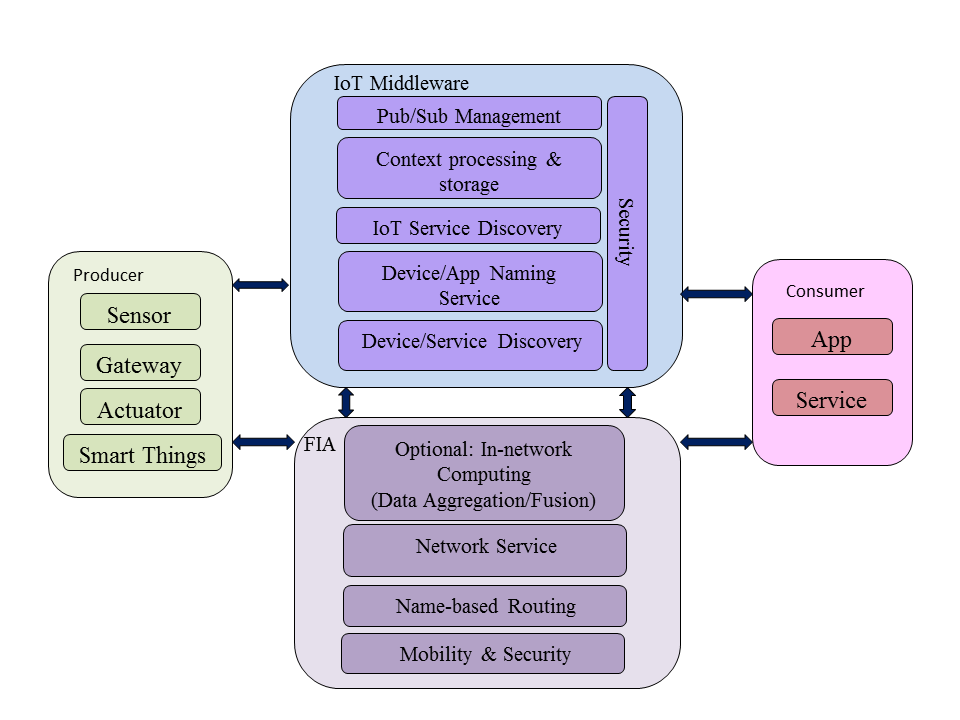
\includegraphics[width=\columnwidth]{figure/middleware_architecture.png}
\caption{\label{fig:mid_arch} ICN-IoT middleware functionality break down.}
\end{figure}
\subsection{Name Data Networking (NDN)}
NDN provides a receiver-driven architecture by transmitting with two types of packets : Interest and Data. Consumer issues Interest of the hierarchical content name and forward to Data Producer. When the interest arrives at the node that own this piece of content, Data Producer will reply with a Data Packet along the reverse path to the Data Consumer. NDN provides three types of key component to support such functionality. Forwarding Information Base (FIB) collects the forwarding information at each NDN node. The content prefix and out-face mapping is recorded in the FIB. Once a certain face receive Data packet for a Pending Interest Table , it could be added into the FIB to indicate a healthy data retrieving path.Pending Interest Table (PIT) is a data structure that maintain the set of pending Interest routed by the node that expecting Data packet in return. PIT entry is created by receiving Interest, and filters the redundant Interest that carried the same content name. Due to the limitation of PIT size, every PIT entry comes with a timeout which is estimated based on a round trip time. Once a matching Data packet being received by the node, it is forwarded via the face recorded in the PIT before this entry being removed. Content Store(CS) is a data cache for storing Data packet for matching Interest along the reverse path. Also, due to the constraint of local CS size, Data Producer can define the freshness of the Data packet in order to timeout it in the cache. With such transmission mechanism, NDN eliminates the notion of source and destination as it is in IP network, and handle routing only for Interest Packet.

\subsection{MobilityFirst Background}\label{sec:intro_mf}
MF utilizes GUID to name every network object, while separating this GUID from its actual network address. This identifier(GUID)/locator(NA) split design allows MF supporting dynamic address binding, multiple addressing binding and late binding. Shown as Figure ~\ref{}, MF core network architecture includes the following network component.

\vspace{1mm}\noindent{\bf Global Name Resolution Service(GNRS)}: GNRS is a centralized service that maintains mappings between GUID and network address. MF routers create the entries by performing an Insert for the GUIDs of attached network devices and the associated network address, and query GNRS for a translation from GUID to latest binding network address. Recent works shows that this translation performance is much better (50-100 ms delay) than DNS resolution~\cite{vu2012dmap}.

\vspace{1mm}\noindent{\bf Hybrid GUID/NA address routing}: Each of the router in MF can make routing decision based on NA or GUID in the header of data packet, since routing decision are made on a hop-by-hop manner~\cite{nelson2011gstar}.

\vspace{1mm}\noindent{\bf Delay-Tolerant Network(DTN)}: The storage in each MF router provides the capability of caching the data packe. Hence, data can be stored or forwarded based on different routing policies, such as quality of the link, which is very useful over wireless interface.
\begin{figure}
\centering
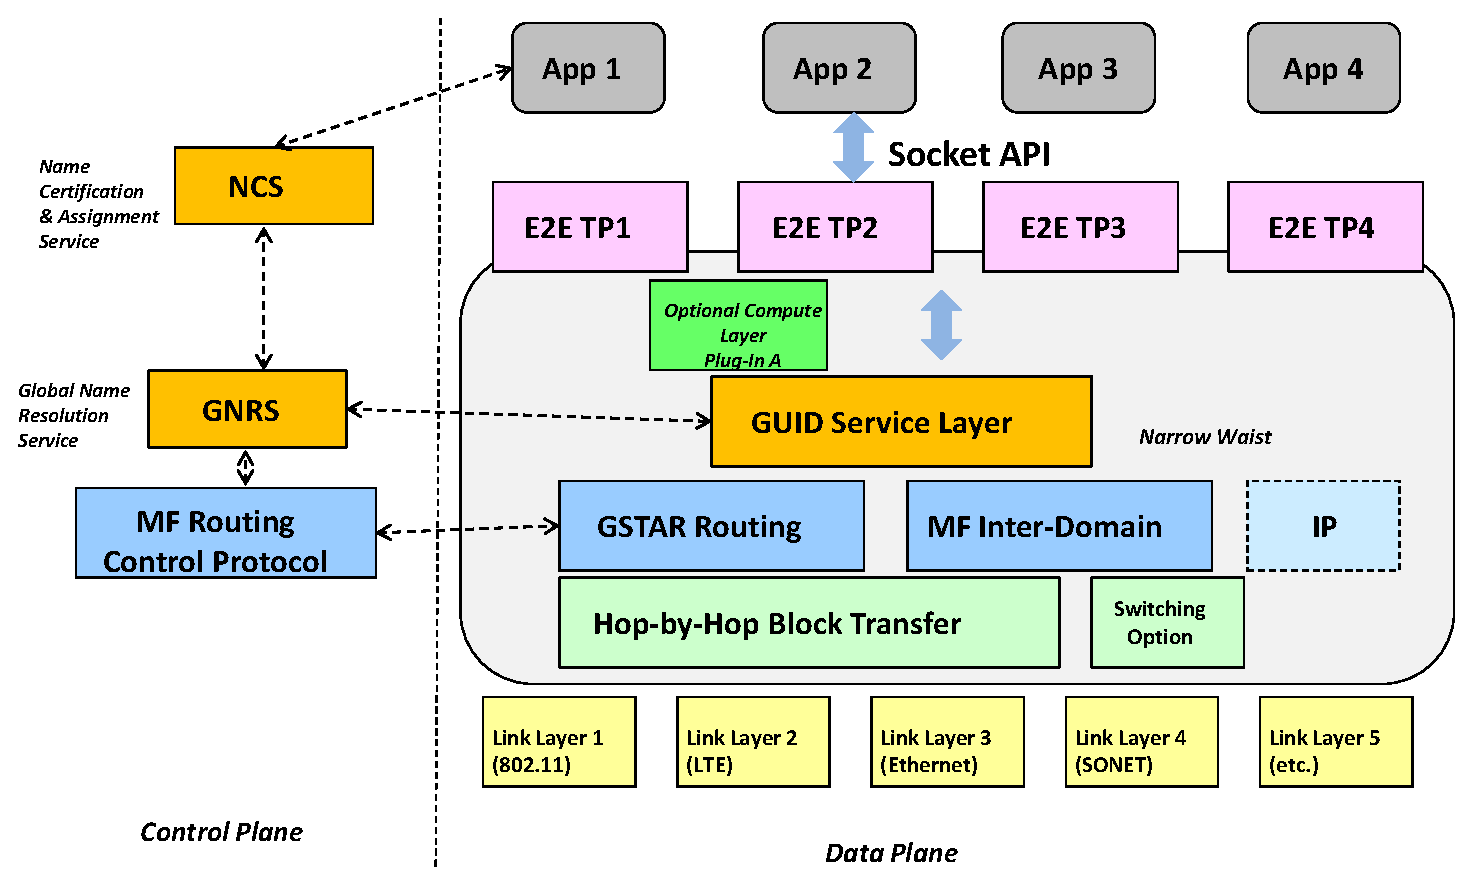
\includegraphics[width=\columnwidth]{figure/mf_arch.eps}
\caption{\label{fig:mf_arch}Mobilityfirst architecture.}
\end{figure}
%\subsection{MF Multicast}\label{sec:multi}

\vspace{1mm}\noindent{\bf MF multicast}MF multicast is based on the idea of group GUID that gathers multiple network objects into one entity. Group GUID  to object GUID mapping is a one-to-many mapping that being maintained at GNRS server. Network object can claim to join the multicast group, and either edge router or a centralized management service will perform insertion of the object GUID to group GUID mapping to into GNRS server. When the first router queries GNRS server for a group GUID mapping, GNRS server returns a list of member GUIDs. The router assembles these GUIDs into the header and performs "Longest Common Path(LCP)" algorithm to determine the next hop address.Shown as Figure~\ref{fig:multicast}, routers look up the routing table for these GUIDs, and check if there are multiple next hops. When the number of result is more than one, the router reassembles the header and forwards the copied packet to corresponding interfaces. If the number of multicast group member become significant, another approach can be adopted to resolve this issue--instead of assembling all GUIDs into the header after one query, each router on the path queries GNRS server for the group members and perform LCP to decide next hop.
\begin{figure}
\centering
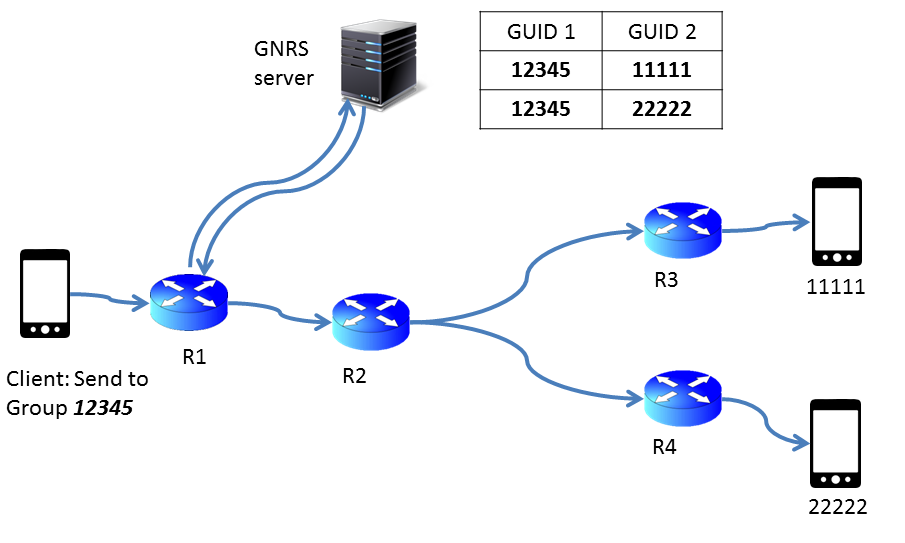
\includegraphics[width=\columnwidth]{figure/multicast.png}
\caption{\label{fig:multicast}MF multicast example: A client send message to Group 12345}
\end{figure}  